
%(BEGIN_QUESTION)
% Copyright 2012, Tony R. Kuphaldt, released under the Creative Commons Attribution License (v 1.0)
% This means you may do almost anything with this work of mine, so long as you give me proper credit

We may analyze the horizontal and vertical ``components'' of an angled force by sketching a right triangle and calculating the lengths of that triangle's sides.  The angled force vector length will be the magnitude of the applied force, while the opposite and adjacent side lengths will represent the horizontal and vertical components of that force.

\vskip 10pt

In this example, we see a person pushing a lawnmower.  The handle of this lawnmower transmits a force of 20 pounds from the person's body to the lanwmower frame, at an angle of 32 degrees from horizontal:

$$\includegraphics[width=15.5cm]{i02068x01.eps}$$

Use trigonometry to calculate how much of this angled force translates into {\it forward} (horizontal) force to drive the lawnmower forward against the friction of the grass, and how much of the applied force translates to {\it downward} (vertical) force pressing the lawnmower wheels against the ground.

\vskip 10pt

$F_{forward} = F_x$ = \underbar{\hskip 50pt} lbs

\vskip 10pt

$F_{down} = F_y$ = \underbar{\hskip 50pt} lbs

\vskip 10pt

If the person doing the lawnmowing wishes to apply their force more efficiently to the mower (i.e. more of their force going into the forward component and less pushing downward), should they hold the lawnmower handle at a shallower angle or at a steeper angle?

\vskip 20pt \vbox{\hrule \hbox{\strut \vrule{} {\bf Suggestions for Socratic discussion} \vrule} \hrule}

\begin{itemize}
\item{} A technique highly recommended for word-problems is to {\it sketch a picture} of the problem and label elements of that picture with the given information.  Do this, and compare your sketch with those of your classmates.  How, specifically, does this aid your problem-solving?
\end{itemize}

\underbar{file i02068}
%(END_QUESTION)





%(BEGIN_ANSWER)

$F_{forward} = F_x$ = (20 lb) (cos 32$^{o}$) = {\bf 16.96 lbs}

\vskip 10pt

$F_{down} = F_y$ = (20 lb) (sin 32$^{o}$) = {\bf 10.60 lbs}

\vskip 10pt

Maximum pushing efficiency will be realized when the person shrinks to the height of the lanwmower deck and is pushing 100\% horizontally (0$^{o}$ angle from the ground).

%(END_ANSWER)





%(BEGIN_NOTES)


%INDEX% Mathematics review: trigonometric calculations

%(END_NOTES)


